\documentclass[tikz,border=2pt]{standalone}
\usepackage{amsmath,amssymb}
\usepackage{pgfplots}
\pgfplotsset{compat=1.18}

\begin{document}
% The sample mean of n i.i.d. observations (sigma = 1) has standard deviation 1/sqrt(n): its
% distribution piles up around mu as n grows, so P(|Xbar_n - mu| > eps) -> 0.
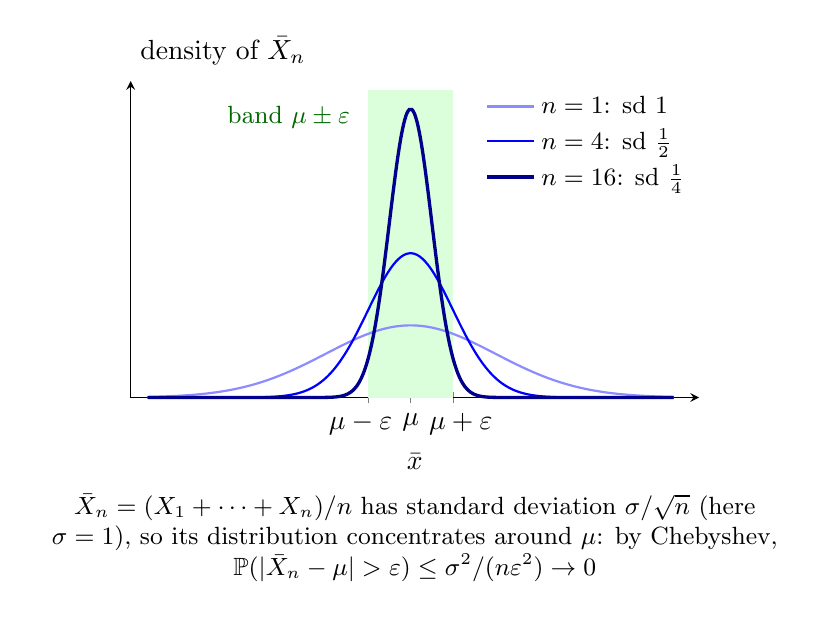
\begin{tikzpicture}
	\begin{axis}[
		axis lines=left, xmin=-3.3, xmax=3.4, ymin=0, ymax=1.75,
		xtick={-0.5,0,0.5}, xticklabels={$\mu-\varepsilon\;\;$,$\mu$,$\;\;\mu+\varepsilon$}, ytick=\empty,
		xlabel={$\bar x$}, ylabel={density of $\bar X_n$}, ylabel style={rotate=-90, anchor=south west, at={(axis description cs:0,1.02)}},
		samples=200, smooth, width=8.8cm, height=5.6cm, clip=false,
		legend style={draw=none, fill=none, font=\small, at={(1.0,0.99)}, anchor=north east}, legend cell align=left
		]
		\fill[green!14] (axis cs:-0.5,0) rectangle (axis cs:0.5,1.7);
		\addplot[blue!45, thick, domain=-3.1:3.1] {exp(-x^2/2)/sqrt(2*pi)};
		\addlegendentry{$n=1$: sd $1$}
		\addplot[blue, thick, domain=-3.1:3.1] {2*exp(-x^2*2)/sqrt(2*pi)};
		\addlegendentry{$n=4$: sd $\tfrac12$}
		\addplot[blue!55!black, very thick, domain=-3.1:3.1] {4*exp(-x^2*8)/sqrt(2*pi)};
		\addlegendentry{$n=16$: sd $\tfrac14$}
		\node[green!40!black, font=\small, anchor=east] at (axis cs:-0.6,1.55) {band $\mu\pm\varepsilon$};
	\end{axis}
	\node[anchor=north, font=\small, align=flush center, text width=9.6cm] at ([yshift=-2pt]current axis.outer south) {$\bar X_n=(X_1+\cdots+X_n)/n$ has standard deviation $\sigma/\sqrt n$ (here $\sigma=1$), so its distribution concentrates around $\mu$: by Chebyshev, $\mathbb{P}(|\bar X_n-\mu|>\varepsilon)\le\sigma^2/(n\varepsilon^2)\to0$};
\end{tikzpicture}
\end{document}
